%!TEX root = ../Main.tex

\section{Methodology and Data}\label{sec:4MethodData}

\subsection{Data and Calculation of Input Factors}\label{sec:41Data}
The data used in this study are from several sources. The realized variance of the S\&P 500 index is obtained from the \textcite{Oxford:RV}. Daily VIX values are the closing values from \gls{CBOE}. As of September 22, 2003 \gls{CBOE} started to use a revised methodology for the VIX, but calculated the prices with the new methodology ex-post, dating back until 1990. Therefore the data was taken both from the ex-post \textcite{CBOE:old} and the daily-updated \textcite{CBOE:new}. The S\&P 500 which is only used for visualisation are closing values also taken from \textcite{SandP}. The sample consists of daily data in the period from January 2000 to December 2017. \\
Firstly, the model needs daily realized volatility, to assess the information content of implied volatilities. The calculation of the daily realized variance is calculated by \textcite{Oxford:RV} using the sum of squared 5-min high-frequency returns, as explained in \ref{sec:221RV}. The formula is given by 
\begin{align}
\sigma_{t} = \sum x_{t}^{2}
\end{align}
with $x_{t} = X_{t} - X_{t-1}$ and $X_{t}$ being the logarithm of the price at time $t$. \\%
Previous research has used different sampling frequencies for the calculation of the realized volatility. Whereas earlier studies used mainly daily returns, most recent studies argue in the favor of using intraday returns, as they have certain advantages over daily data \parencite{jiang2003}. For example \textcite{andersen2003} point out that high-frequency returns help both for predicting again high-frequency returns, but also that they contain information for longer horizons, such as monthly or quarterly. Moreover and more importantly, \textcite{andersen1998} show that realized volatility calculated using squared returns produces inaccuracies when daily retruns are used. The reaqlized variace data is cleaned by \textcite{Oxford:RV} in four ways. First, entries outside the timestamp when exchanges are open are deleted. Secondly, entries with the same time stamp are replaced with the median bid-ask price. Thirdly entries with a negative spread (as they violate the no-arbitrage condition) or extremely large spread (50 times the median of the day) are deleted. Lastly, entries for which the mid-quote deviated largely from the mean where deleted. To obtain the realized volatility, the realized variance is simply squared
\begin{align}
RV_{t} = \sqrt{(\sum x_{t}^{2})}.
\end{align}
Moreover, the model needs historic volatility, to capture the information contained in the past realized volatility. Therefore simply lagged realized volatiltiy is used. 
Finally, the VIX is needed to measure the information contained in this model-free implied volatiltiy measure. For the VIX the daily closing value is taken, as it contains the information from the whole day. The calculation is described in \ref{sec:223VIX}. To display the data in a more intuitive manner, the annualized VIX is divided by the square root of 252 as in \textcite{blair2001} and \textcite{whaley2008}, in order to obtain an index with daily information content.\\
The S\&P 500 together with the VIX is illustrated in \ref{fig1} and the realized vola is added in \ref{fig2}. The summary statistics can be found in \ref{tab:summary1} and \ref{tab:sumamry2} in the appendix. The summary statistics show, that the mean of the VIX is for every time period a slightly higher than the mean of the realized variance for all time periods. From the graphics, too, it can be seen that usually the VIX is a little higher than the realized volatility. This is consistent with the findings previous research, e.g. \textcite{jiang2003}. However, during crisis periods, the realized volatility exceeds the VIX. For example, whereas both the realized volatility and the VIX are particularly high during the period of the crisis between 2008 and 2012, the realized variance is significantly higher. To account for this period, a dummy was included in the model.\\ Moreover the summary statistics show, that the skewness and kurtosis of the logarithmic specification is closer to the one of the normal distribution. Consequently, a regression based on the log volatilities is also specified and should be statistically better specified than those based on simple volatility. \\
The correlation matrix for the realized volatility, it's lagged specifications and the model-free implied volatility and it's lags can be found in \ref{tab:corr1}. Overall, the realized volatility is highly correlated with both the past realized variance and the past VIX values. Whereas for the one day lag the correlation with the VIX is higher, for the weekly and monthly averages the correlation with the realized variance is higher. 


\begin{figure}[!htbp]\label{fig1}
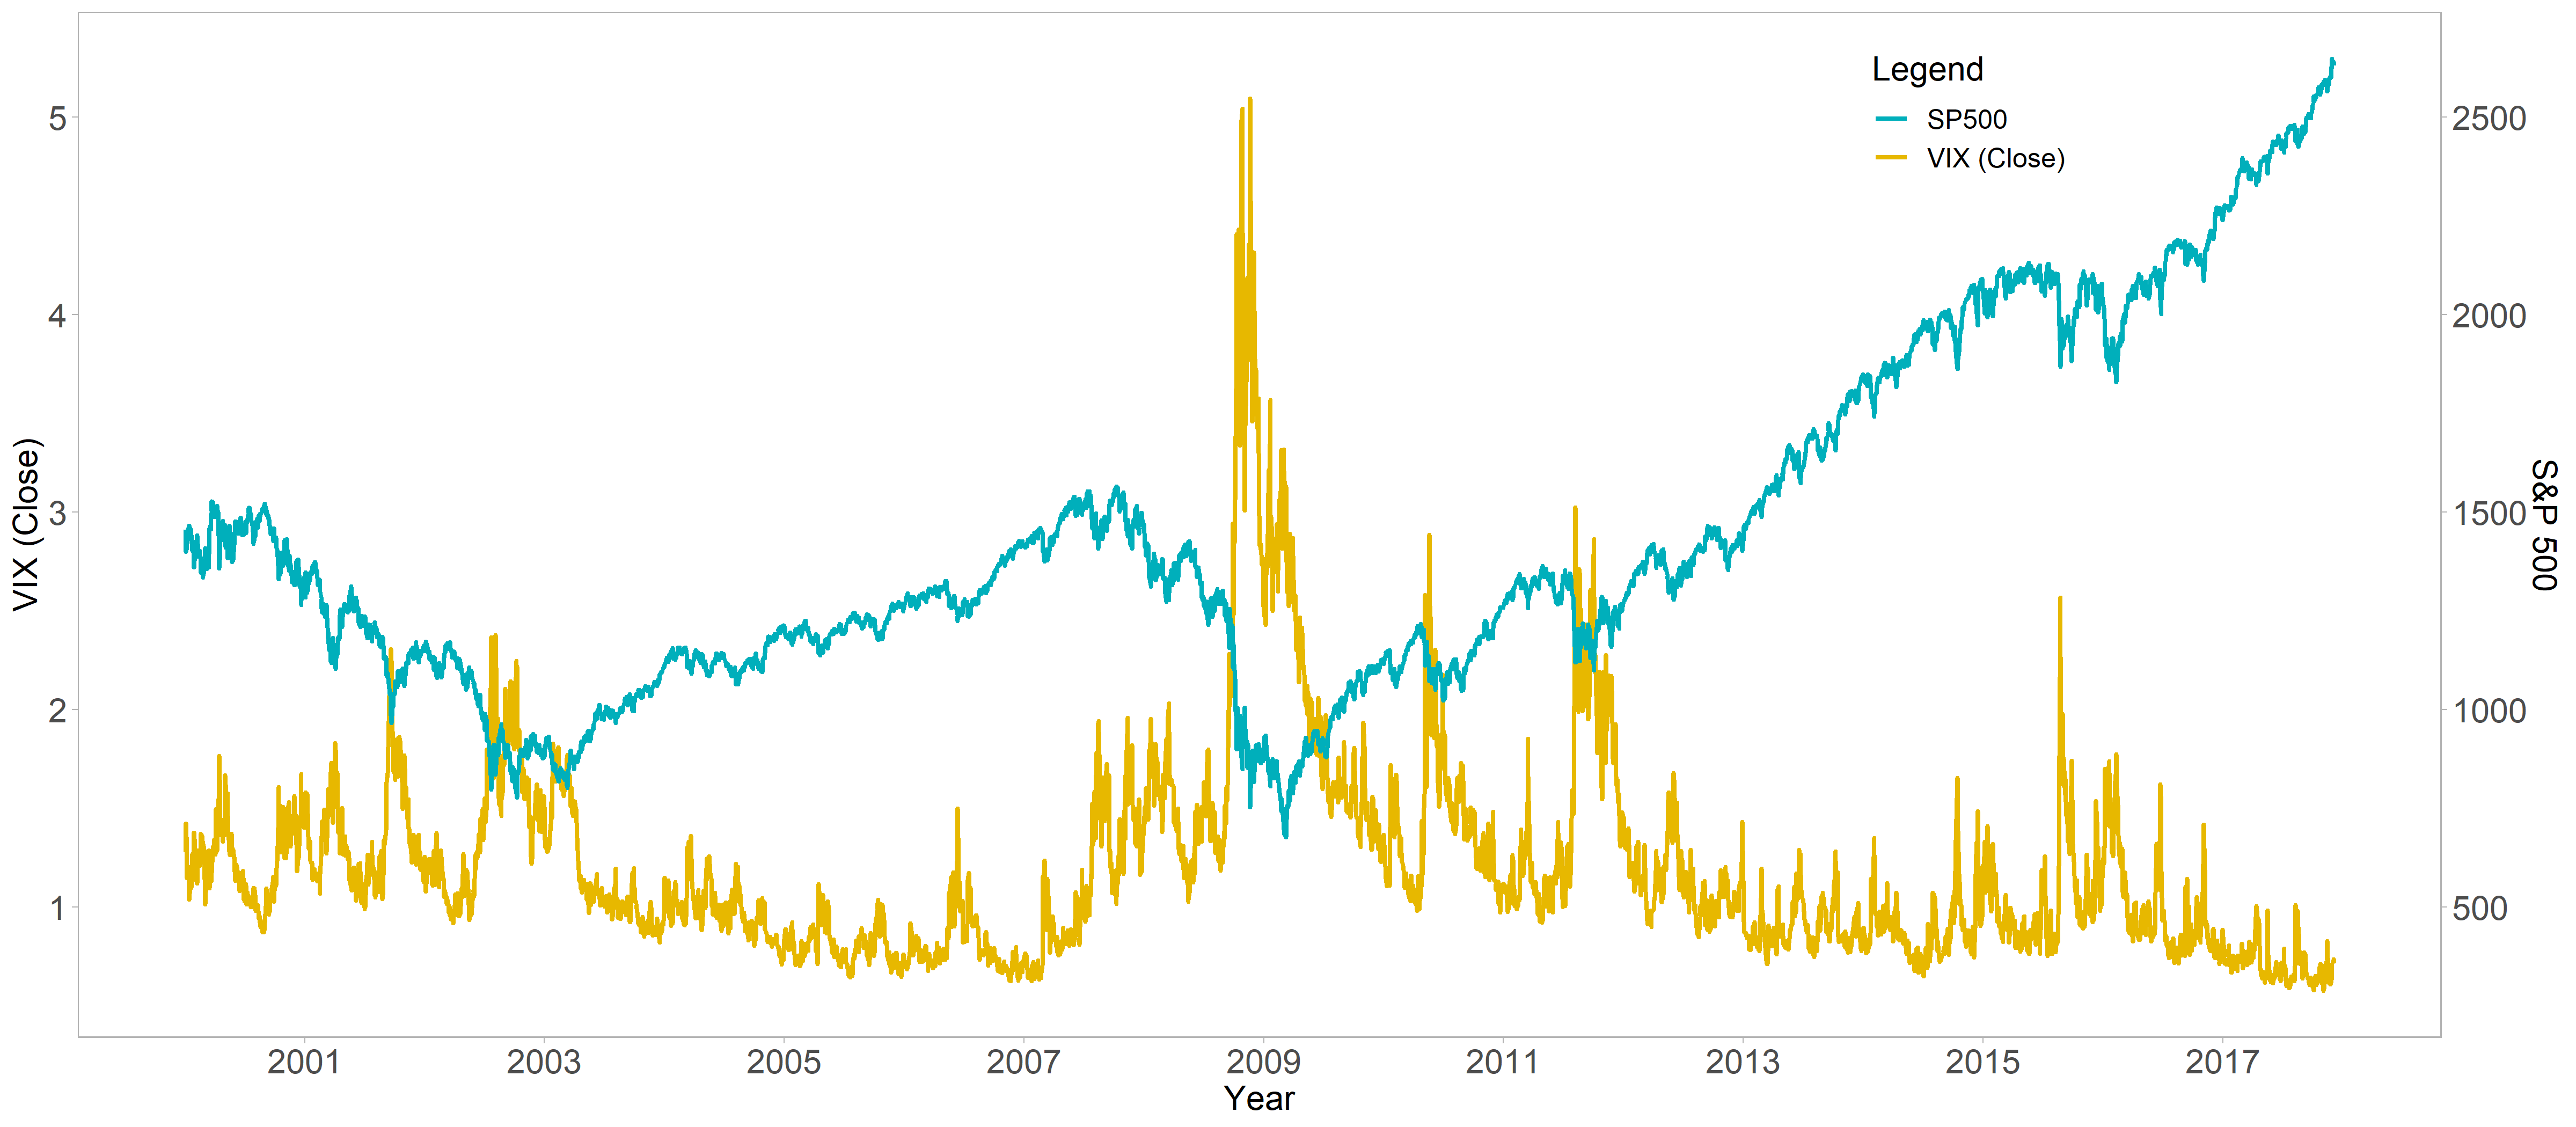
\includegraphics[width=16cm, height=8cm]{pictures/SPandViX.png}
\end{figure}

\begin{figure}[!htbp]\label{fig2}
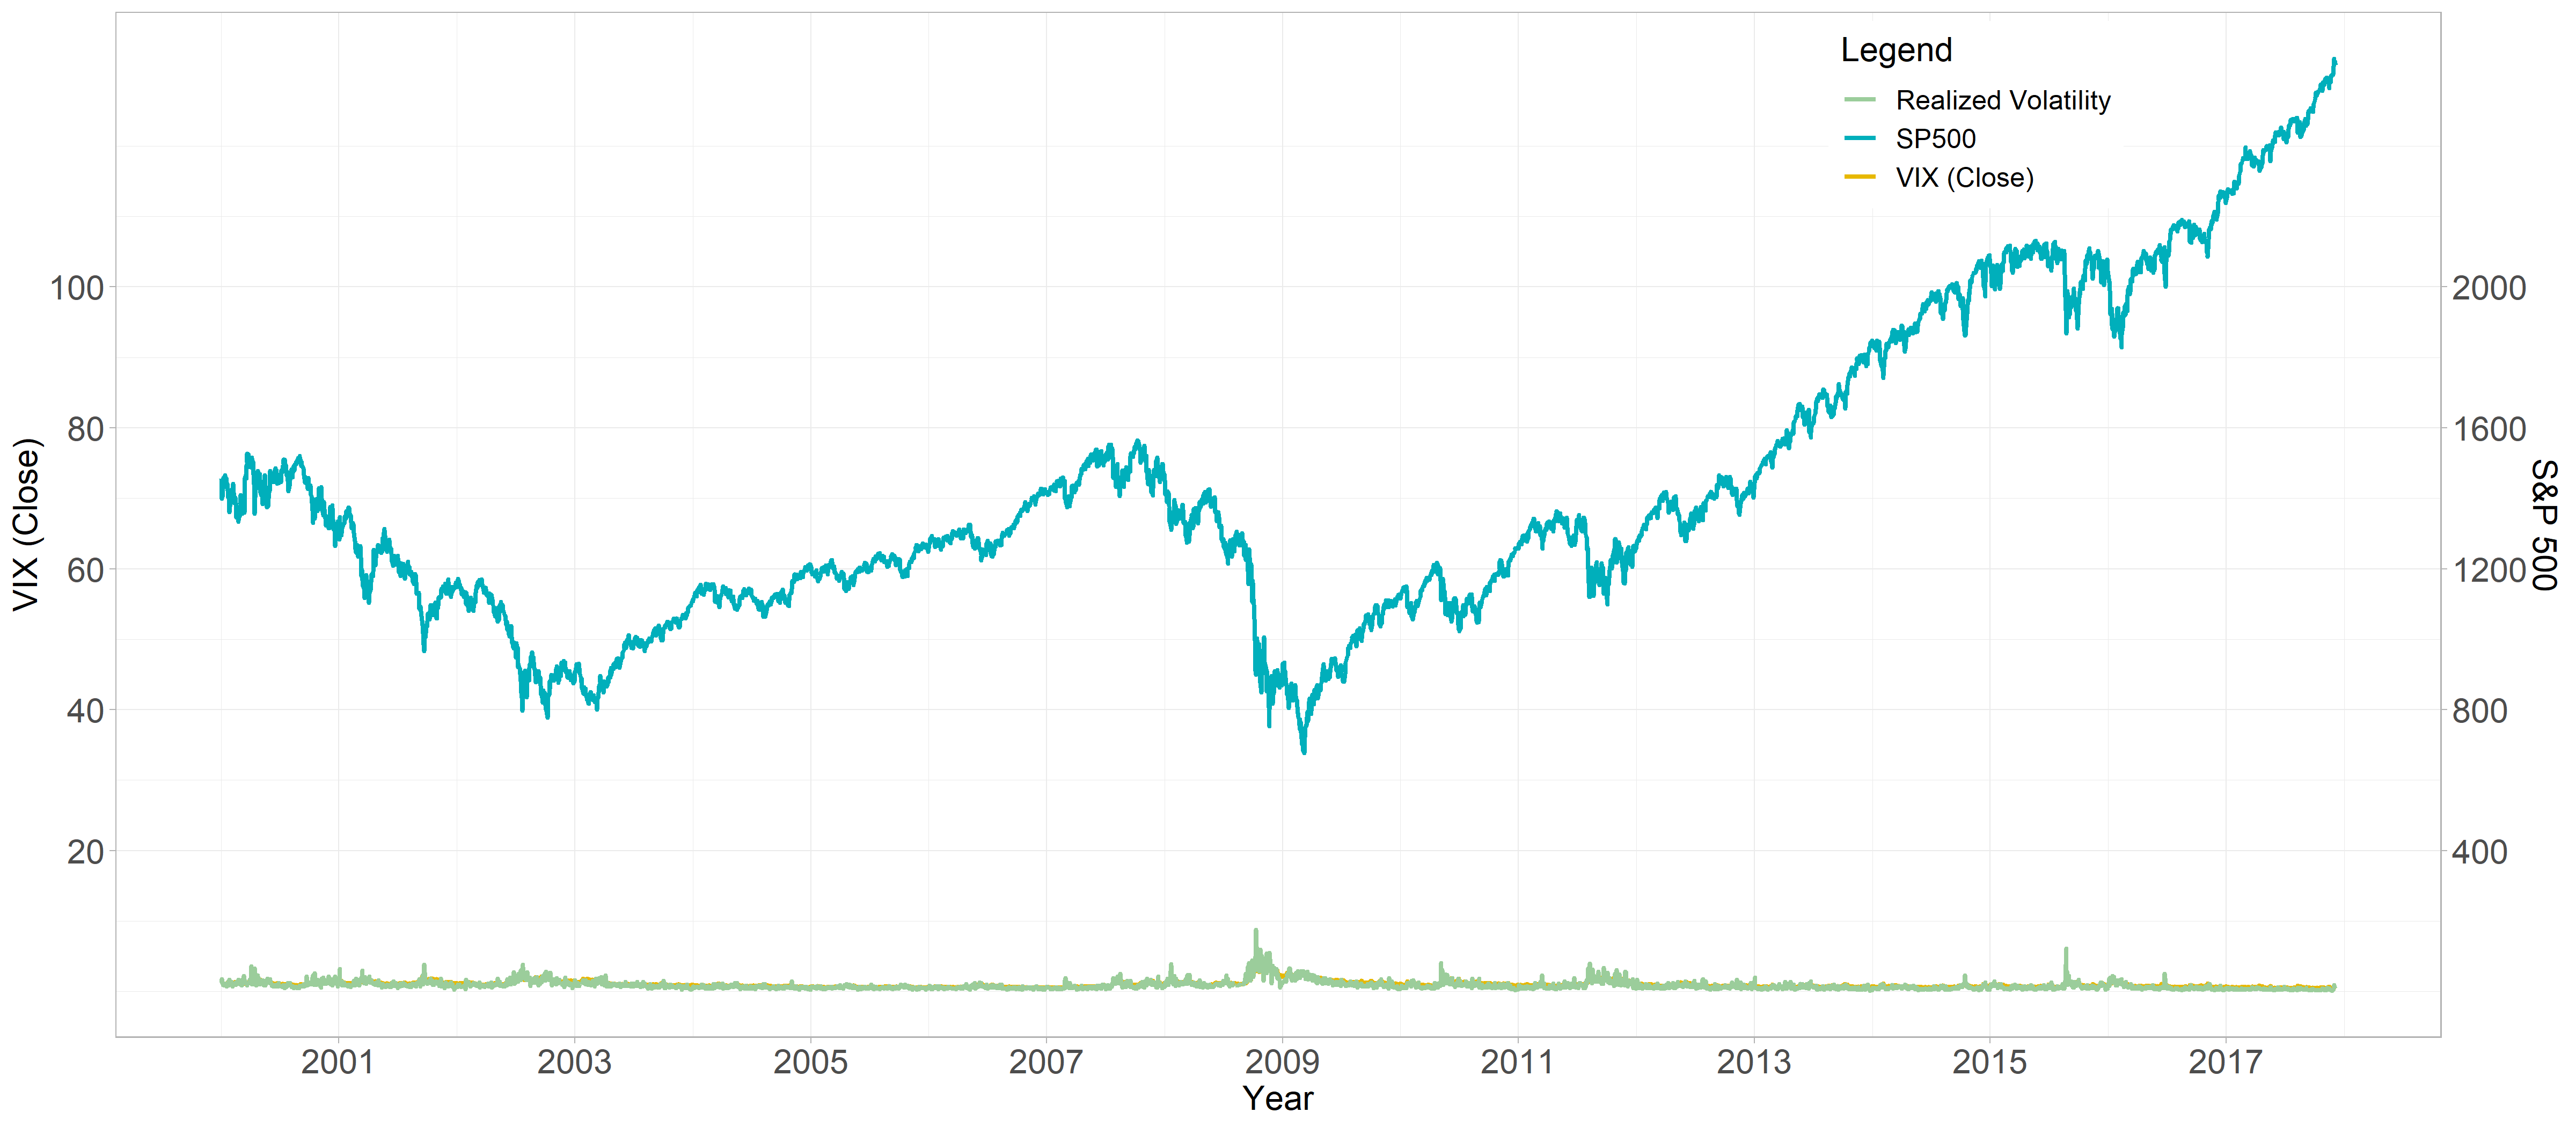
\includegraphics[width=16cm, height=8cm]{pictures/SPandVolandViX.png}
\end{figure}


\subsection{Methodology: Linear Regression and HAR-RV model}\label{sec:42Method}
Consistent with prior research, for example \textcite{jiang2003}, \textcite{canina1993} or \textcite{christensen1998}, both univariate and encompassing regression analysis is used to analyse the information content of volatility measures. However, contrary to previous research, the approach from the HAR-RV model, described by \textcite{Corsi2009} is used. This means, not only one day lagged realized volatility is included as an explanatory variable in the regression, but also weekly and monthly realized volatility. They are computed using simply rolling averages, the weekly volatility is the average over 5 days and the monthly volatility the average over 22 days.\\
In the univariate regression, the realized volatility is regressed once only on the historic data, and once only on the VIX. For comparison, realized volatility is regressed on both historic data and the VIX in the encompassing regression analysis. Thus the encompassing regression analysis gives information about the relative importance of the volatility measures, and whether the VIX subsumes the information from the historic volatility. For each explanatory variable, the value of the current day $t$ is used, whereas for the explained variable, the one-day-ahead value $t+1d$ is used. Like this, all the information available on day $t$ is used to evaluate the volatility one day ahead. The three regressions are then given by:
\begin{align}\label{eq:myregression}
RV_{t+1d} &= c + \beta^{d} RV^{d}_{t} + \beta^{w} RV^{w}_{t} + \beta^{m} RV^{m}_{t}  \\
RV_{t+1d} &= c + \beta^{VIX} VIX_{t} \\
RV_{t+1d} &= c + \beta^{d} RV^{d}_{t} + \beta^{w} RV^{w}_{t} + \beta^{m} RV^{m}_{t} + \beta^{VIX} VIX
\end{align}
with $RV_{t+1d}$ the realized volatiltiy one day ahead, $RV^{d}$ the daily realized volatility (lagged compared to the explained variable), $RV^{w}_{t}$ the weekly realized volatility, $RV^{m}_{t}$ the monthly realized volatility, $VIX$ the VIX closing value and $crisis$ the dummy variable, indicating one in the time of the financial crisis (2008-2012) and zero otherwise. The same regressions are specified with the logarithm for each variable.\\
In alignment with \textcite{corsi2009}, the Newey-West covariance correction is used, to account for the possible presence of serial correlation in the data, as serial correlation causes both the Gauss-Markow and Classical linear model assumptions to fail. \\
The hypothesis described in \ref{sec:32Hypothesis} are then formalized in the following way. For \textbf{Hypothesis 1}, if model-free implied volatility contains information about realized volatility, the $H_{0}: \beta^{VIX} = 0$ is should be tested in the regression containing only the VIX and the crisis dummy (with the expectation to be rejected). For the \textbf{Hypothesis 2}, the $H_{0}: \alpha = 0 \ and \ \beta^{VIX} = 1$ should be tested in the same regression (with the expectation to be not rejected). For the \textbf{Hypothesis 3}, that the VIX has more explanatory power than the historical volatility in estimating future realized volatility, the adjusted $R^{2}$s and AIC should be compared in Regressions containing only the VIX or only historic volatility and the crisis dummy. Finally, for \textbf{Hypothesis 4}, that the VIX incorporates all information regarding future realized volatility and that historic volatility contains no incremental information compared to the VIX, the $H_{0}: \beta^{d} = \beta^{w} = \beta^{m} = 0 \ and \ \beta^{VIX} = 1$ shall be tested (expected to not be rejected). 



\subsection{Limitations}\label{sec:43Limits}
As volatility is stochastic, the ex-ante estimation will not equal the return volatility, as it is a measurement over an aggregated discrete time period \parencite{andersen2001}.
The VIX might be flawed, as \textcite{jiang2007} showed.
There might be a bias in estimated realized volatility due to autocorrelation in intraday returns \parencite{jiang2003}. 
